% Metódy inžinierskej práce

\documentclass[10pt,twocolumn,twoside,slovak,a4paper]{article}
\usepackage{wrapfig}
\usepackage{amsmath}
\usepackage[slovak]{babel}
%\usepackage[T1]{fontenc}
\usepackage[IL2]{fontenc} % lepšia sadzba písmena Ľ než v T1
\usepackage[utf8]{inputenc}
\usepackage{graphicx}
\usepackage{url} % príkaz \url na formátovanie URL
\usepackage{hyperref} % odkazy v texte budú aktívne (pri niektorých triedach dokumentov spôsobuje posun textu)
\usepackage{subcaption}

\usepackage{cite}
%\usepackage{times}

\pagestyle{headings}

\title{Získavanie dát a strojové učenie v oblasti kyberbezpečnosti\thanks{Semestrálny projekt v predmete Metódy inžinierskej práce, ak. rok 2023/24, vedenie: Richard Marko}} % meno a priezvisko vyučujúceho na cvičeniach

\author{Kristián Kapec\\[2pt]
	{\small Slovenská technická univerzita v Bratislave}\\
	{\small Fakulta informatiky a informačných technológií}\\
	{\small \texttt{xkapeck@stuba.sk}}
	}

\date{\small 28.september 2023} % upravte



\begin{document}

\maketitle

\begin{abstract}
V tejto modernej a digitálnej dobe je veľmi dôležité chránenie citlivých údajov a dát. Práve na tieto účely nám slúži získavanie dát, ktoré umožňuje zbierať a analyzovať informácie o útokoch, na základe ktorých môže strojové učenie automaticky identifikovať hrozby v reálnom čase, čím sa zvyšuje úroveň bezpečnosti a ochrany dát.  V tomto článku zhodnotíme stav týchto technológií v súčasnosti, ich efektívnosť a rýchlosť detekcie hrozieb. V článku sa taktiež zameriame na výzvy späté s týmito technológiami a pozrieme sa aj na ich možný budúci vývoj . Technológie sa neustále zlepšujú a preto je veľmi dôležité aby aj tieto ochranné prvky napredovali dopredu aby nás dokázali ochrániť aj pred novými hrozbami
\end{abstract}



\section{Úvod}

Motivujte čitateľa a vysvetlite, o čom píšete. Úvod sa väčšinou nedelí na časti.

Uveďte explicitne štruktúru článku. Tu je nejaký príklad.
Základný problém, ktorý bol naznačený v úvode, je podrobnejšie vysvetlený v časti~\ref{nejaka}.
\begin{wrapfigure}{l}{0.2\textwidth}

\includegraphics[width=0.2\textwidth]{STU-FIIT-zfv.png}
 \centering
\end{wrapfigure}
Dôležité súvislosti sú uvedené v častiach~\ref{dolezita} a~\ref{dolezitejsia}.
Záverečné poznámky prináša časť~\ref{zaver}.


\section{Nejaká časť} \label{nejaka}
\begin{figure}[h!]
\centering
\begin{subfigure}[b]{0.4\linewidth}
  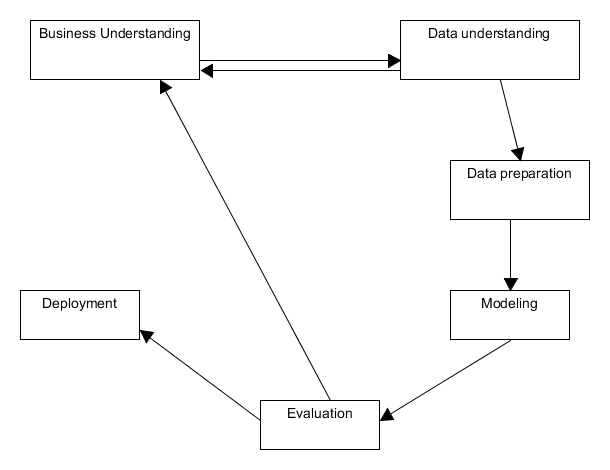
\includegraphics[width=\linewidth,angle=45]{diagram1.png}
  \caption{ Diagram1}
  \label{fig:Diagram1}
\end{subfigure}
\begin{subfigure}[b]{0.4\linewidth}
  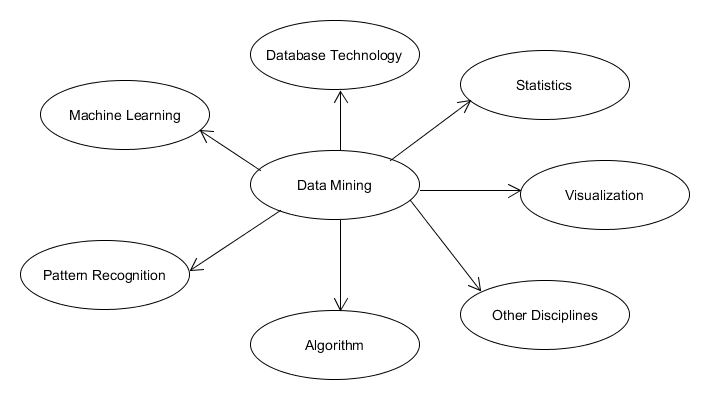
\includegraphics[width=\linewidth]{diagram2.png}
  \caption{ Diagram2}
  \label{fig:Diagram2}
\end{subfigure}
\end{figure}
\begin{figure}[b]
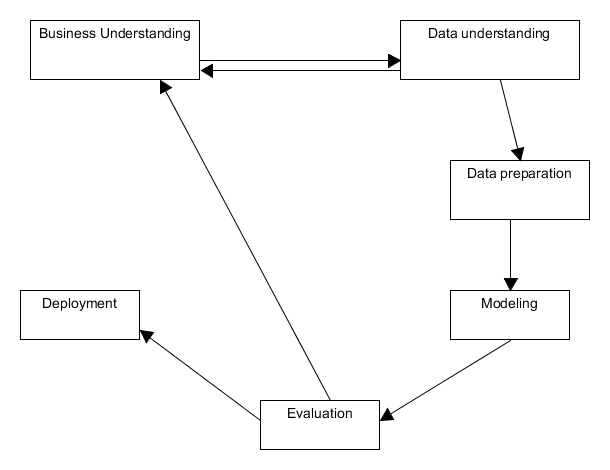
\includegraphics[scale=0.4]{diagram1.png}
  \caption{ Diagram1}
  \label{fig:Diagram1}
\end{figure}

Z obr.~\ref{f:rozhod} je všetko jasné. 

\begin{figure*}[tbh]
\centering
%\includegraphics[scale=1.0]{diagram.pdf}
Aj text môže byť prezentovaný ako obrázok. Stane sa z neho označný plávajúci objekt. Po vytvorení diagramu zrušte znak \texttt{\%} pred príkazom \verb|\includegraphics| označte tento riadok ako komentár (tiež pomocou znaku \texttt{\%}).
\caption{Rozhodujúci argument.}
\label{f:rozhod}
\end{figure*}



\section{Iná časť} \label{ina}
$\begin{bmatrix}
1 & 2 & 3 & 4 & 5\\
5 & 4 & 3 & 2 & 1\\
4 & 3 & 2 & 1 & 5\\
1 & 2 & 5 & 4 & 1\\
 1& 1 & 1 & 1 & 1

\end{bmatrix}$


det(A) =
(-1)1+1 * a11 * A11 + (-1)1+2 * a12 * A12 + (-1)1+3 * a13 * A13 + (-1)1+4 * a14 * A14 + (-1)1+5 * a15 * A15


Základným problémom je teda\ldots{} Najprv sa pozrieme na nejaké vysvetlenie (časť~\ref{ina:nejake}), a potom na ešte nejaké (časť~\ref{ina:nejake}).\footnote{Niekedy môžete potrebovať aj poznámku pod čiarou.}

Môže sa zdať, že problém vlastne nejestvuje\cite{Coplien:MPD}, ale bolo dokázané, že to tak nie je~\cite{Czarnecki:Staged, Czarnecki:Progress}. Napriek tomu, aj dnes na webe narazíme na všelijaké pochybné názory\cite{PLP-Framework}. Dôležité veci možno \emph{zdôrazniť kurzívou}.


\subsection{Nejaké vysvetlenie} \label{ina:nejake}

Niekedy treba uviesť zoznam:

\begin{itemize}
\item jedna vec
\item druhá vec
	\begin{itemize}
	\item x
	\item y
	\end{itemize}
\end{itemize}

Ten istý zoznam, len číslovaný:

\begin{enumerate}
\item jedna vec
\item druhá vec
	\begin{enumerate}
	\item x
	\item y
	\end{enumerate}
\end{enumerate}


\subsection{Ešte nejaké vysvetlenie} \label{ina:este}

\paragraph{Veľmi dôležitá poznámka.}
Niekedy je potrebné nadpisom označiť odsek. Text pokračuje hneď za nadpisom.



\section{Dôležitá časť} \label{dolezita}




\section{Ešte dôležitejšia časť} \label{dolezitejsia}




\section{Záver} \label{zaver} % prípadne iný variant názvu



%\acknowledgement{Ak niekomu chcete poďakovať\ldots}


% týmto sa generuje zoznam literatúry z obsahu súboru literatura.bib podľa toho, na čo sa v článku odkazujete
%\bibliography{literatura}

\bibliographystyle{plain} % prípadne alpha, abbrv alebo hociktorý iný
\end{document}
